% personal latex template

% vegito2002@gmail.com
\documentclass{article}
\usepackage{times}
\usepackage{mathptmx}
\usepackage{multirow}
\usepackage{enumitem}
\usepackage[letterpaper, margin=1in]{geometry}
\usepackage{hyperref}
\usepackage{amsmath}
\usepackage{mathtools}
\DeclarePairedDelimiter{\ceil}{\lceil}{\rceil}
\DeclarePairedDelimiter{\floor}{\lfloor}{\rfloor}
\usepackage{graphicx}
\usepackage{listings}
\usepackage{lipsum}
\usepackage{courier}
% \usepackage{tabularx}
\usepackage[export]{adjustbox}
% \usepackage[landscape]{pdfpages}
\usepackage{enumitem}
\usepackage{spreadtab}
% \usepackage{enumerate}


\graphicspath{ {images/} }

\usepackage[dvipsnames]{xcolor}  %% Allow color names
\lstset
{ %Formatting for code in appendix
  belowcaptionskip=1\baselineskip,
  xleftmargin=\parindent,
  language=Java,   %% Change this to whatever you write in
  breaklines=true, %% Wrap long lines
  basicstyle=\ttfamily,
  % numbers=left,
  % stepnumber=1,
  commentstyle=\itshape\color{Gray},
  stringstyle=\color{Orange},
  keywordstyle=\bfseries\color{WildStrawberry},
  identifierstyle=\color{Blue},
}
\usepackage{titlesec}
\usepackage{amssymb}
\newenvironment{claim}[1]{\par\noindent\underline{Claim:}\space#1}{}
\newenvironment{claimproof}[1]{\par\noindent\underline{Proof:}\space#1}{\leavevmode\unskip\penalty9999 \hbox{}\nobreak\hfill\quad\hbox{$\blacksquare$}}

\setcounter{secnumdepth}{4}

\titleformat{\paragraph}
{\normalfont\normalsize\bfseries}{\theparagraph}{1em}{}
\titlespacing*{\paragraph}
{0pt}{3.25ex plus 1ex minus .2ex}{1.5ex plus .2ex}

\begin{document}

% Article top matter
\title{\textsc{EN 600.425 Declarative Methods \\ - Term Project Writeup}\\ \textbf{\textsc{Better } \texttt{diff}}} %\LaTeX is a macro for printing the Latex logo
\author{Guoye Zhang, Qiang Zhang\\
        % \texttt{Hopkins ID: 92CC3E}
        }  %\texttt formats the text to a typewriter style font
\date{\today}  %\today is replaced with the current date
\maketitle

\section{Introduction}
The utility \texttt{diff} is commonly used in all scenarios, whether for programming purpose or in general text editing circumstances. The website Github integrated \texttt{diff} into their version control system, facilitating ubiquitous knowledge of the utility. This legacy utility is based on the renowned \textit{Edit Distance} algorithm, which in essence is a Dynamic Programming algorithm. \\

Aside from the application domain of version control, \texttt{diff}'s algorithm in itself is interesting and instructive enough for most computer science students to delve into. In general sense, the concepts of finding similar text and displaying minimum edit distance can be embodied in various domains and categories of applications. Our project aims at extending \texttt{diff} to provide firstly the feature of multi-file editting source referencing, accompanied with visualization, that can display the chain of editting among more than two files placed in the same folder, together with a better algorithm that fixes a certain scenario where the normal \texttt{diff}'s Edit Distance algorithm would perform suboptimally, which is a case we already described in the proposal.\\

\subsection{Algorithmic Optimization}
As a reminder, recall the scenario where normal \texttt{diff} would perform suboptimally. In this code snippet:\\
\begin{lstlisting}
   for(int i=0; i<10; i++) {
       System.out.println("First line");
   }
   for(int i=0; i<10; i++) {
       System.out.println("Second line");
   }
   for(int i=0; i<10; i++) {
       System.out.println("Third line");
   }
\end{lstlisting}
from which we will delete the second \texttt{for} block. And if we use the traditional \texttt{diff} on the old and new versions of this snippet, we would get:\\
\begin{lstlisting}
   for(int i=0; i<10; i++) {
       System.out.println("First line");
   }
   for(int i=0; i<10; i++) {
 -     System.out.println("Second line");
 - }
 - for(int i=0; i<10; i++) {
       System.out.println("Third line");
   }
\end{lstlisting}
Instead of what would be expecting as follows:
\begin{lstlisting}
   for(int i=0; i<10; i++) {
       System.out.println("First line");
   }
 - for(int i=0; i<10; i++) {
 -     System.out.println("Second line");
 - }
   for(int i=0; i<10; i++) {
       System.out.println("Third line");
   }
\end{lstlisting}
This case is fixd with our improved version of \texttt{diff} algorithm, which we shall call by \texttt{MDiff} in the rest of this document. In fact, there are much more scenarios where the traditional \texttt{diff} algorithm would disappoint you. For example, consider the instance of comparison below (results are hand-generalized from Github's webpage highlighting):
\begin{lstlisting}
<a><b>
 ----

<b><a>
 ++++
\end{lstlisting}
The notations used here should be self-explanatory. When comparing the two strings of \texttt{<a><b>} and \texttt{<b><a>}, traditional \texttt{diff} would return the results as shown above, which means, in a 0-based indexing convention, deleting the 1-4 of the first string, and adding the 4 characters at index 1-4 of the second string. But this answer of editting distance is clearly suboptimal. The optimal solution we expect would be:
\begin{lstlisting}
<a><b>
 -  -

<b><a>
 +  +
\end{lstlisting}
which is the answer that \texttt{MDiff} would return.

\subsection{Multi-file Referencing}
In this part, we extended \texttt{diff} to another domain of applicaiton of interest. To most eyes, \texttt{diff} is generally used to comparing the editting distance between two files. It is a utility used widely in use. Indeed, it is a utility, in that it does a job well, but it is not typically tailored for any domain. We implemented an application that embodies \texttt{MDiff} in its core, but meanwhile provides far more convenient and appleasing functionalities. \\

For oft, we are interested not only to know the difference between two text files. Rather, we want to be able to look at some paragraph of this text file, and find out from which other paragraph in other file this paragraph derives. Text reusing is so common nowadays that this is a feature of no trivial productivity significance. In fact, to fullfill such a task, of finding the ancestor of a paragraph in this text file, most people would resort to nothing better than a brute-force file-by-file \textit{Open\&Search} routine. \\

To implement this feature, the optimized algorithm of \texttt{MDiff} alone is not quite enough. In practical scale, even comparing only two files with a \texttt{diff}-based algorithm can be undesirably slow. Not to mention that we are trying to determine edit chains between multiple files. For the application to be fast enough to be useful in practice, certain techniques are used to structure the implementation of its functionality.\\

The use case we are trying to address here is a scenario where the folder contains, rather than multiple files, multiple versions of a file. For example, \texttt{file1} could be the original file of an article in craft. Then after certain modifications, \texttt{file2} results. In the end, the folder contains multiple files, each pair of which, albeit being different, shares an overall similarity larger than 50\%. Aside from that, we make the below assumptions:
\begin{enumerate}
  \item File name indicate each file's last-modified-by time in an increasing order. Thus if there is a file $i$ and a file $j$ with $i<j$, we can convince ourselves that file $i$ is lastly modified earlier than file $j$ and file $j$ is thus possile a successor of $i$: meaning we should include file $i$'s texts when we try to search for the ancestor of any text paragraph in file $j$. To be honest, this modelling is not perfectly accurate. For example, in the case below:\\
  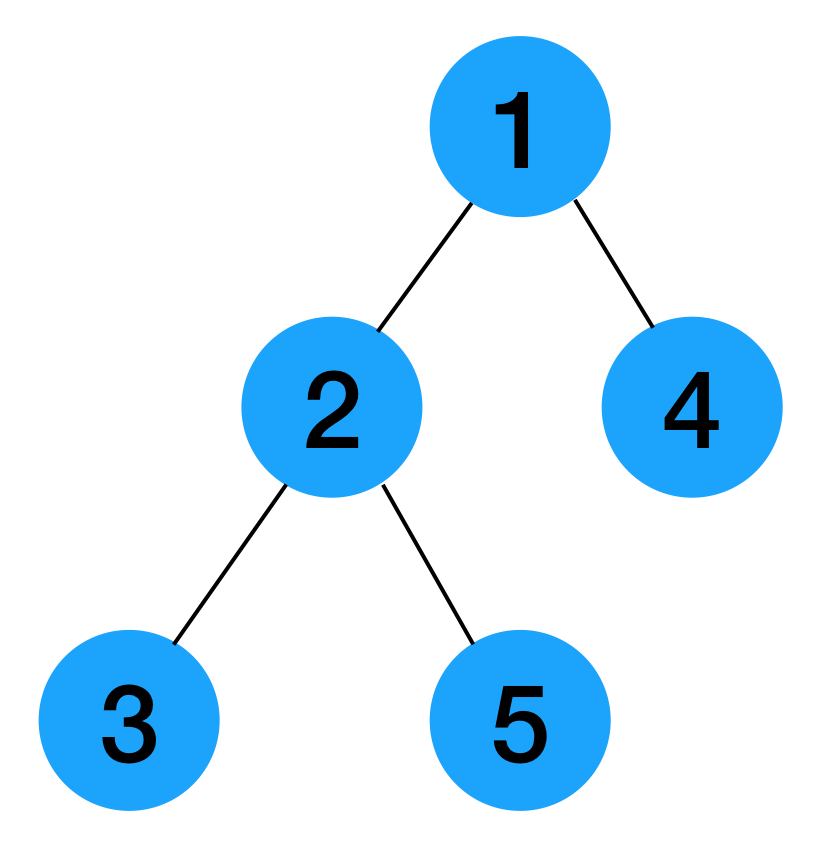
\includegraphics[scale=0.3,center]{pic1.png}

  File 5 is modified later than file 4 (since 5 is larger than 4, and thus file 5 has a later last modification timestamp), but file 5 actually should not consider file 4 as one of its ancestor, because file 5 comes from modifications of file 2, and is on a editting path branch disjoint from that of file 2. 

  But overall, our approach should work fine. 
  \item The author of the files knows to seperate each section, or paragraph of his files by an empty line. Like:
  \begin{lstlisting}
  <paragraph1>

  <paragraph2>

  <paragraph3>
  \end{lstlisting}
  This is similar to how most Latex users format their documents. 
\end{enumerate}
When we open a certain file $i$, we want to be able to know:
\begin{enumerate}
  \item \textbf{Objective 1}: Amongst all the paragraphs of all files in this folder, which paragraph is most likely to be the direct predecessor of this paragraph? Or, which paragraph is most likely to be the direct source of modification for this paragraph?
  \item \textbf{Objective 2}: After finding the most likely predecessor of this paragraph, what are the minimum amount of edits required to change from the predecessor paragraph to the paragraph under inspection?
\end{enumerate}

Objective 2 as we described in the last subsection, is addressed by an optimized version of \texttt{diff} algorithm, which we call \texttt{MDiff}. Objective 1's on the other hand, is key to speeding up the application to a speed suitable for real-life utilization. \\

By matching texts in the unit of paragraph first, we largely reduced the computational effort required. Yet this scheme does not violate any practical editting convention to render the application infutile. Normally, when a user edits a file, the edits, however many there are at a time, can be each bucketted into its own paragraph. By matching paragraphs first, we limit the scope to apply \texttt{MDiff} on to only a paragraph a time.  This is analogous to an idea in 3D game designing that you don't have to render the entire 3D scene and maintain it at all time. You just have to render as large as the player's camera can capture and only when the camera does captures it. This optimization can reduce the computational cost of the application by a factor as large as several hundreds inpractice. \\

The key idea behind implementing Objective 1, and the paragraph matching explained above, is determine textual similarities. There is a well-established technique called Min-hash which is used to calculate a text document's signature, which can in turn be used to compare with another document's signature to determine the similarity between the two documents. Of course, we here are looking at the similarity between two documents rather than two paragraphs. We used a third-party library \cite{minhash} which can return the similarity of two text strings based on the Min-hash algorithm. \\

There are more subtlties to be clarified in this scheme. But we are leaving further elaboration for later part of this document. 

\subsection{Running Instruction}
By this point, enough information is provided to understand what this project hopes to deliver. In this section, we provide step by step instructions so that you can run the application now and see the results before going further. 

\section{First Step: Finding the Most Similar Paragraph}
As described in the previous section, our first goal is to be able to inspect a certain file $i$ in the folder, and immediately locate the most similar paragraph amongst all files in the folder, under assumptions:
\begin{enumerate}
  \item File name indicate each file's last-modified-by time in an increasing order.
  \item The author of the files knows to seperate each section, or paragraph of his files by an empty line. 
\end{enumerate}

The second assumption is established so that there is a valid way to define the notion of ancestry. If we treat an entire document as one single paragraph, then there is no point in saying \textit{finding the ancestor of this entire document}. Because in practice, most modifications between files are minor and of comparable degree, which means different successors of the same predecessor document may end up looking very much alike. Even though we devise an algorithm to locate such an ancestor document for the document being inspected, the output is most likely to be inaccurate and uninformative. \\

After dividing a document into paragraphs, the notion of ancestry and the concept of reusing now makes sense. Think it this way: when you write code, if you say \textit{reuse}, you usually refers to reusing a part of a code file, usually a function, or block. But in the case you want to reuse the code file in its entirety, you just \texttt{import} or \texttt{include} it. Such file-wise reusing operations would normally indicate the source of reusing directly and an dedicated algorithm to solve the ancestry relationship would be unnecessary. The same analysis applies to the case of general text files. We are only interested in finding the predecessor of a snippet of a text file, which is a reused part. We conveniently define such a concept of reused part as a paragraph. There can be other choices of delimitation of reused parts, but obsession over this definition is moot per se. \\

Now, to find the most likely ancestor of a paragraph, is to find a paragraph that:
\begin{enumerate}
  \item is contained in a file that is lastly modified earlier than the file that contains the paragraph under inspection.
  \item shares, amongst all paragraphs that satisfies the previous condition, a highest similarity with the paragraph under inspection.
  \item owns a similarity with the paragraph that satisfies the previous condition that is higher than a lower threshold.
\end{enumerate}
And to find such a paragraph that satisfies the above three conditions, we use the theory of textual similarity. In particular, we implement the process as follow:
\begin{enumerate}
  \item
\end{enumerate}

















\begin{thebibliography}{9}
%The \bibitem is to start a new reference.  Ensure that the cite_key is
%unique.  You don't need to put each element on a new line, but I did
%simply for readability.
    \bibitem{minhash}
      \href{https://github.com/codelibs/minhash}{codelibs/minhash: A third-party Java-based libary  for b-bit MinHash algorism}


\end{thebibliography} %Must end the environment


\end{document}  %End of document.